\documentclass[answers,11pt]{exam}
\usepackage[spanish]{babel}
\usepackage[utf8]{inputenx}
\usepackage{fontenc}
\usepackage{textcomp}
\usepackage{lmodern,pifont}
\usepackage{graphicx}
\usepackage{setspace}
\usepackage[dvipsnames]{color}
\usepackage{colortbl}
\usepackage{caption}
\usepackage{amsmath}

\renewcommand{\solutiontitle}{\noindent\textbf{Solución:}\par\noindent}
\pagestyle{empty}
\begin{document}
{\fontfamily{lmss}\selectfont
\textbf{INSTRUCCIONES:}
\begin{itemize}
    \item Se dispone de dos horas para responder las 20 preguntas. 10 por cada unidad formativa
    \item Cada pregunta tiene un valor de 1 punto.
    \item Para aprobar el modulo es necesario aprobar cada unidad formativa,
      esto es, se ha de obtener una puntuación mínima de 5 puntos en cada unidad
      formativa 
    \item Para considerar la respuesta como correcta, la opción escogida ha de
      estar correctamente señalada. Las preguntas erróneamente marcadas se
      considerarán como incorrectas. 
    \item Cada respuesta incorrecta resta 0.33 puntos. Las respuestas en blanco no restan. 
\end{itemize}
\vspace{1cm}


  \textbf{UF 0008. Instalaciones agrarias. Mantenimiento limpieza y
    desinfección.}

\begin{questions}
  \question La luz desarrolla un papel fundamental en el ciclo vegetativo de las
    plantas. La luz influye en funciones tales como...
    \begin{checkboxes}
      \choice A. Fotosíntesis, fotoperiodismo, fototropismo y transpiración
      \choice B. Transpiración, floración y fructificación
      \choice C. Crecimiento y desarrollo de plagas y enfermedades
      \CorrectChoice D. Las respuestas A y B son correctas
    \end{checkboxes}

    \question Las diferentes fases de un cultivo en un invernadero están
    condicionadas por cuatro factores ambientales o climáticos. Señala la opción
    correcta.
    \begin{checkboxes}
      \choice A. Topografía, humedad, temperatura y latitud
      \CorrectChoice B. Temperatura, humedad relativa, luz y concentración de
     $CO_2$
      \choice C. Temperatura, humedad del suelo, orientación y luminosidad
      \choice D. Topografía, viento dominante, humedad y tipo de invernadero
    \end{checkboxes}

  \question Según la cantidad de horas de luz que una planta puede recibir, ¿las
    plantas de día largo...?
    \begin{checkboxes}
      \choice A. Requieren de pocas horas de luz para florecer
      \CorrectChoice B. Requieren de pocas horas de oscuridad para florecer
      \choice C. Requieren de muchas horas de oscuridad para florecer
      \choice D. Ninguna es correcta
    \end{checkboxes}
    
  \question Los métodos para corregir los niveles de humedad consumen agua,
    ¿puedes indicar que métodos pueden usarse para ahorrar agua e influir en el
    nivel de humedad de un invernadero?
    \begin{checkboxes}
      \choice A. Sistemas de goteo
      \CorrectChoice B. Acolchados y sombreados
      \choice C. Sistemas de ventilación forzada
      \choice D. Sistemas de micro-nebulización
    \end{checkboxes}
    
  \question ¿Cuando decimos que un conductor que lleva corriente toca otro cable
    o parte del circuito, nos referimos a que se ha producido un?
    \begin{checkboxes}
      \CorrectChoice A. Cortocircuito
      \choice B. Sobrecarga
      \choice C. Chispazo
      \choice D. Todas son correctas
    \end{checkboxes}
    
  \question Señala que precauciones se deben tomar para realizar el mantenimiento
    de instalaciones agrícolas?
    \begin{checkboxes}
      \choice A. Seleccionar herramientas y útiles adecuados
      \choice B. Comprobar correcto funcionamiento de la maquinaria después del
      mantenimiento
      \choice C. Eliminación de residuos de productos y subproductos de las
      labores de mantenimiento
      \CorrectChoice D. Todas son correctas
    \end{checkboxes}

  \question De las siguientes medidas señala la que NO es una medida física de
    lucha para la desinsectación
    \begin{checkboxes}
      \choice A. Colocar mosquiteras
      \CorrectChoice B. Empleo de insecticidas 
      \choice C. Sellar grietas, oquedades y hendiduras
      \choice D. Extremar medidas de limpieza
    \end{checkboxes}

  \question Los equipos de protección respiratoria los clasificamos en dos
    grandes grupos.
    \begin{checkboxes}
      \choice A. Mascarillas desechables y no desechables
      \CorrectChoice B. Equipos filtrantes y equipos aislantes
      \choice C. Equipos de línea de aire y equipos autónomos
      \choice D. De presión positiva y filtrantes
    \end{checkboxes}

  \question ¿Qué tipo de señales tienen forma triangular con fondo amarillo y
    bordes negros?
    \begin{checkboxes}
      \CorrectChoice A. Advertencia de peligro
      \choice B. De obligación
      \choice C. De prohibición
      \choice D. De equipos contra incendios
    \end{checkboxes}
\newpage
  \question ¿Qué señala la imagen siguiente? (El pictograma es negro sobre fondo
    amarillo)
  \begin{figure}[h!]
    \centering
    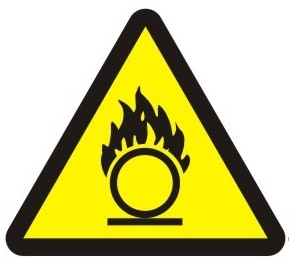
\includegraphics[scale= 0.6]{images/combustible.jpg}
  \end{figure}
  \begin{checkboxes}
    \CorrectChoice A. Peligro material combustible
    \choice B. Prohibido encender fuego
    \choice C. Peligro atrapamiento
    \choice D. Peligro de incendio
  \end{checkboxes}

  
\newpage  
\textbf{UF 0009. Mantenimiento, preparación y manejo de tractores}  
\question ¿En cuantas partes podemos dividir visualmente un motor de combustión interna? 
\begin{checkboxes}
\choice A. 4 partes. Carter, culata, filtros y volante de inercia
\choice B. 3 partes. Carter, cilindros y embrague 
\CorrectChoice C. 3 partes. Carter, bloque motor y tapa de culata
\choice D. 4 partes. Carter, culata, motor de arranque y radiador    
\end{checkboxes}

\question ¿Generalmente que tipo de refrigeración lleva el motor de un tractor?
\begin{checkboxes}
\choice A. De aire
\choice B. De aire o de agua
\choice C. De ventilación forzada
\CorrectChoice D. De agua
\end{checkboxes}

\question El sistema de engrase de un motor de 4T, ¿es importante controlar la
  presión de este sistema?
\begin{checkboxes}
\choice A. No se controla la presión del sistema de engrase
\CorrectChoice B. Si. Es muy importante y se controla mediante un manómetro o testigo luminoso
\choice C. El sistema de engrase del motor no necesita supervisión
\choice D. El sistema de engrase es importante para el motor pero no hay manera de controlarlo
\end{checkboxes}

\question Si un motor de combustión interna no tiene sistema de engrase, ¿qué tipo de motor es?
\begin{checkboxes}
\choice A. De un motor que utiliza \emph{gasoil} como combustible
\CorrectChoice B. Motor de dos tiempos
\choice C. Todos los motores tienen un sistema de engrase
\choice D. Ningúna es correcta
\end{checkboxes}

\question Si en el cilindro de un motor diesel de 4t, encontramos las válvulas
  de admisión y escape cerradas, ¿en  qué tiempos y carrera puede estar el
  motor? 
\begin{checkboxes}
\CorrectChoice A. Carrera ascendente de compresión o carrera descendente de expansión 
\choice B. Carrera ascendente de admisión o carrera descendente de escape
\choice C. Carrera descendente de expansión o carrera descendente de admisión
\choice D. Carrera ascendente de compresión o carrera ascendente de escape
\end{checkboxes}

\question ¿Qué tipo de estructuras de protección antivuelco existen para tractores?
\begin{checkboxes}
\choice A. Solo cabinas
\CorrectChoice B. Bastidor de dos postes, bastidor de cuatro postes y cabina
\choice C. Bastidor de dos y cuatro postes
\choice D. Cabina cerrada
\end{checkboxes}
\newpage
\question Para hacer una limpieza de bornes de batería, ¿cual es el orden en el
  que hay que retirar los cables para desconectarla? 
\begin{checkboxes}
\CorrectChoice A. Primero el cable del borne negativo y despues el positivo
\choice B. Primero el positivo y despues el negativo
\choice C. Retiramos los dos a la vez
\choice D. No hay que retirar los cables para desconectarla, simplemente quitar
las llaves del contacto 
\end{checkboxes}

\question ¿Qué es recomendable hacer antes de poner en marcha un tractor que no
  conocemos y ponemos en funcionamiento por primera vez? 
\begin{checkboxes}
\CorrectChoice A. Leer el manual del fabricante
\choice B. Comprobar niveles
\choice C. Comprobar en la hoja de vida el mantenimiento realizado
\choice D. Comprobar que no hay tornillos sueltos
\end{checkboxes}

\question La estructura anti-vuelco de un tractor, ¿imposibilita que un tractor
  pueda sufrir un vuelco? 
\begin{checkboxes}
\choice A. Si. Están diseñadas para que impidan el vuelco de un tractor
\choice B. Si, pero han de emplearse medidas de seguridad complementarias como
el cinturon de seguridad
\choice C. Si, pero solo si es una cabina
\CorrectChoice D. No. No están diseñados para impedir la posibilidad de vuelco,
solo para minimizar la gravedad de las lesiones en caso de accidente 
\end{checkboxes}

\question ¿Qué medidas de protección son adecuadas para los puntos de engranaje?
\begin{checkboxes}
\choice A. No operar la máquina sin que las protecciones de estos puntos no estén colocadas
\choice B. Conocer dichos puntos, localizarlos y evitar aproximarse a ellos
cuando la máquina esté en funcionamiento 
\choice C. No realizar ningúna intervención cuando la máquina o alguna de sus
partes esté en movimiento 
\CorrectChoice D. Todas son correctas
\end{checkboxes}

\end{questions}}

\end{document}

%%% Local Variables:
%%% mode: latex
%%% TeX-master: t
%%% End:
